\let\negmedspace\undefined
\let\negthickspace\undefined
\documentclass[journal]{IEEEtran}
\usepackage[a5paper, margin=10mm, onecolumn]{geometry}
\usepackage{tfrupee} 
\setlength{\headheight}{1cm} 
\setlength{\headsep}{0mm}       
\usepackage{gvv-book}
\usepackage{gvv}
\usepackage{cite}
\usepackage{amsmath,amssymb,amsfonts,amsthm}
\usepackage{algorithmic}
\usepackage{graphicx}
\usepackage{textcomp}
\usepackage{xcolor}
\usepackage{txfonts}
\usepackage{listings}
\usepackage{enumitem}
\usepackage{mathtools}
\usepackage{gensymb}
\usepackage{comment}
\usepackage[breaklinks=true]{hyperref}
\usepackage{tkz-euclide} 
\usepackage{listings}
\def\inputGnumericTable{}                                 
\usepackage[latin1]{inputenc}                                
\usepackage{color}                                           
\usepackage{array}                                           
\usepackage{longtable}                                       
\usepackage{calc}                                            
\usepackage{multirow}                                        
\usepackage{hhline}                                          
\usepackage{ifthen}                                          
\usepackage{lscape}
\renewcommand{\thefigure}{\theenumi}
\renewcommand{\thetable}{\theenumi}
\setlength{\intextsep}{10pt} 

\numberwithin{equation}{enumi}
\numberwithin{figure}{enumi}
\renewcommand{\thetable}{\theenumi}

\begin{document}
	
	\bibliographystyle{IEEEtran}
	\vspace{3cm}
	
	\title{4.7.50}
	\author{EE25BTECH11052 - Shriyansh Kalpesh Chawda}
	\maketitle
	\textbf{Question}:\\
	Find the vector equation of the line passing through (1, 2, 3) and perpendicular to the $\vec{r}\cdot(\hat{i} + 2\hat{j} - 5\hat{k}) + 9 = 0$.
	\\
	\textbf{Solution}\\
The plane is given by
		\begin{equation}
			\mathbf r \cdot \brak{1, 2, -5} + 9 = 0
		\end{equation}
		so the plane's normal vector is
		\begin{equation}
			\mathbf n = \myvec{1 \\ 2 \\ -5}.
		\end{equation}
		The required line is perpendicular to the plane, so its direction vector lies in the row space. Thus, the line direction vector can be chosen as
		\begin{equation}
			\mathbf d = \mathbf n = \myvec{1 \\ 2 \\ -5}.
		\end{equation}
Using the point
		\begin{equation}
			\mathbf a = \myvec{1 \\ 2 \\ 3},
		\end{equation}
		the vector equation of the line is
		\begin{equation}
			\mathbf r = \mathbf a + t\mathbf d
		\end{equation}
		\begin{equation}
			\mathbf r = \myvec{1 \\ 2 \\ 3} + t \myvec{1 \\ 2 \\ -5}, \quad t \in \mathbb R.
		\end{equation}
		\begin{figure}[h!]
			\centering
			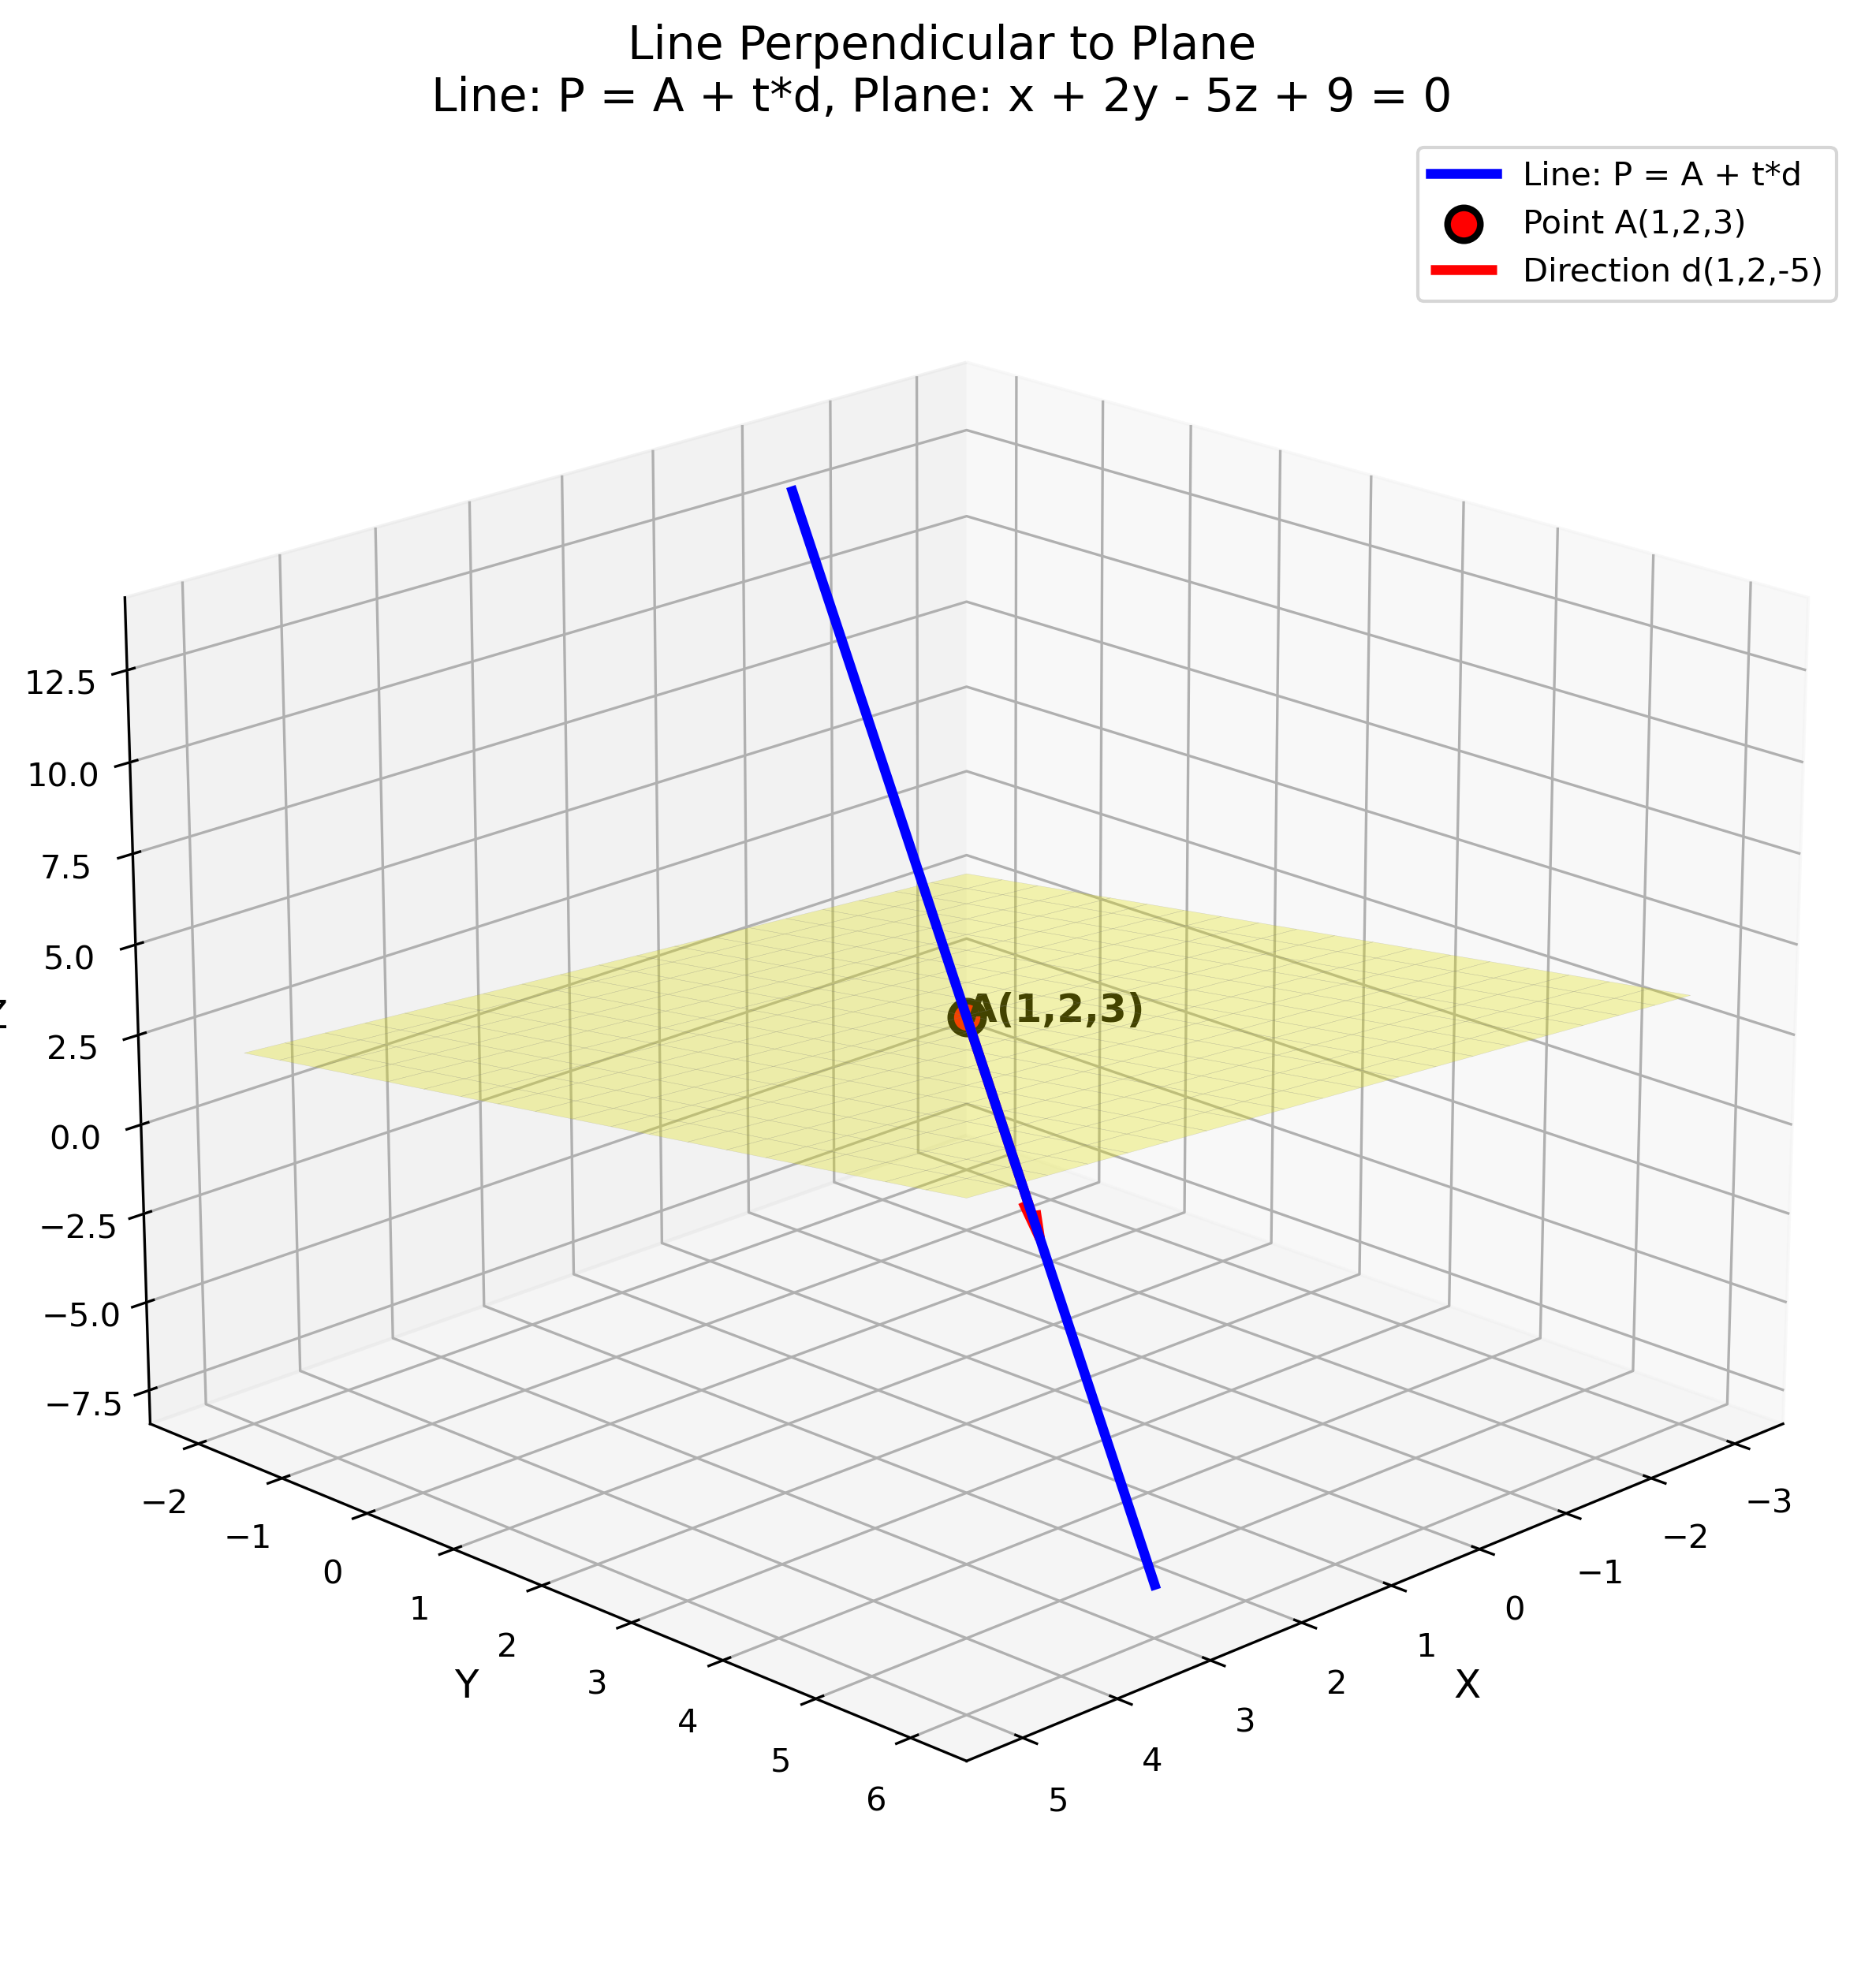
\includegraphics[width=0.9\linewidth]{figs/line_perpendicular}
			\caption{}
			\label{fig:lineperpendicular}
		\end{figure}
		
	\end{document}






\end{document}